% !TEX program = xelatex
\documentclass[11pt,a4paper]{article}
\usepackage[utf8]{inputenc}
\usepackage[T1]{fontenc}
\usepackage[french]{babel}
\usepackage[left=1cm,right=1cm,top=1.2cm,bottom=1.2cm]{geometry}
\usepackage{amsmath}
\usepackage{amssymb}
\usepackage{array}
\usepackage{graphicx}
\usepackage{xcolor}
\usepackage{titlesec}
\usepackage{enumitem}
\usepackage{multicol}
\usepackage{pifont}
% Badges « Exercice n » en cursive Playwrite FR Moderne (police du site),
% chargée à 85 % de la taille courante (XeLaTeX ou LuaLaTeX ; gras sous pdfLaTeX).
\makeatletter
\ifdefined\XeTeXrevision\def\ExoFont@ok{}\fi
\ifdefined\directlua\def\ExoFont@ok{}\fi
\ifdefined\ExoFont@ok
\newcommand{\ExoFont}{\font\ExoFont@f="[../polices/PlaywriteFRModerne.ttf]" at \dimexpr\f@size pt*85/100\relax\ExoFont@f}
\else
\newcommand{\ExoFont}{\bfseries}
\fi
\makeatother
% \ExoTexte{...} : texte du badge en cursive, avec la hauteur d'une majuscule de la
% police courante (la cursive est plus haute et ferait grandir chaque badge).
\newcommand{\ExoTexte}[1]{\raisebox{0pt}[\fontcharht\font`E][0pt]{\ExoFont #1}}
\usepackage{frcursive}
% Correctif du bug de crénage de frcursive sous XeLaTeX (repris de CLT2627.sty) :
% sans lui, certaines paires de lettres consécutives dans \cursive explosent
% (une lettre projetée loin à droite), ce qui coupe des mots comme "Représenter".
\makeatletter
\ifdefined\XeTeXcharclass
\XeTeXcharclass `a 201 \XeTeXcharclass `b 201 \XeTeXcharclass `c 201
\XeTeXcharclass `d 201 \XeTeXcharclass `e 201 \XeTeXcharclass `f 201
\XeTeXcharclass `g 201 \XeTeXcharclass `h 201 \XeTeXcharclass `i 201
\XeTeXcharclass `j 201 \XeTeXcharclass `k 201 \XeTeXcharclass `l 201
\XeTeXcharclass `m 201 \XeTeXcharclass `n 201 \XeTeXcharclass `o 201
\XeTeXcharclass `p 201 \XeTeXcharclass `q 201 \XeTeXcharclass `r 201
\XeTeXcharclass `s 201 \XeTeXcharclass `t 201 \XeTeXcharclass `u 201
\XeTeXcharclass `v 201 \XeTeXcharclass `w 201 \XeTeXcharclass `x 201
\XeTeXcharclass `y 201 \XeTeXcharclass `z 201
\XeTeXcharclass `A 201 \XeTeXcharclass `B 201 \XeTeXcharclass `C 201
\XeTeXcharclass `D 201 \XeTeXcharclass `E 201 \XeTeXcharclass `F 201
\XeTeXcharclass `G 201 \XeTeXcharclass `H 201 \XeTeXcharclass `I 201
\XeTeXcharclass `J 201 \XeTeXcharclass `K 201 \XeTeXcharclass `L 201
\XeTeXcharclass `M 201 \XeTeXcharclass `N 201 \XeTeXcharclass `O 201
\XeTeXcharclass `P 201 \XeTeXcharclass `Q 201 \XeTeXcharclass `R 201
\XeTeXcharclass `S 201 \XeTeXcharclass `T 201 \XeTeXcharclass `U 201
\XeTeXcharclass `V 201 \XeTeXcharclass `W 201 \XeTeXcharclass `X 201
\XeTeXcharclass `Y 201 \XeTeXcharclass `Z 201
\XeTeXcharclass `\é 201 \XeTeXcharclass `\è 201 \XeTeXcharclass `\ê 201
\XeTeXcharclass `\ë 201 \XeTeXcharclass `\É 201 \XeTeXcharclass `\È 201
\XeTeXcharclass `\Ê 201 \XeTeXcharclass `\Ë 201 \XeTeXcharclass `\à 201
\XeTeXcharclass `\â 201 \XeTeXcharclass `\ä 201 \XeTeXcharclass `\À 201
\XeTeXcharclass `\Â 201 \XeTeXcharclass `\Ä 201 \XeTeXcharclass `\ô 201
\XeTeXcharclass `\ö 201 \XeTeXcharclass `\Ô 201 \XeTeXcharclass `\Ö 201
\XeTeXcharclass `\î 201 \XeTeXcharclass `\ï 201 \XeTeXcharclass `\Î 201
\XeTeXcharclass `\Ï 201 \XeTeXcharclass `\ù 201 \XeTeXcharclass `\û 201
\XeTeXcharclass `\ü 201 \XeTeXcharclass `\Ù 201 \XeTeXcharclass `\Û 201
\XeTeXcharclass `\Ü 201 \XeTeXcharclass `\ç 201 \XeTeXcharclass `\Ç 201
\XeTeXcharclass `\œ 201 \XeTeXcharclass `\Œ 201 \XeTeXcharclass `\æ 201
\XeTeXcharclass `\Æ 201
\let\cursive@orig\cursive
\renewcommand{\cursive}{%
  \cursive@orig
  \XeTeXinterchartoks 201 201 = {\kern0pt }%
}
\fi
\makeatother
\usepackage{tikz}
\usetikzlibrary{calc,arrows.meta}
\usepackage{tcolorbox}
\tcbuselibrary{skins,breakable}
\usepackage[hidelinks]{hyperref}
\definecolor{calcblue}{HTML}{1C7ED6}
\definecolor{diffgreen}{HTML}{40C057}
\definecolor{diffblue}{HTML}{228BE6}
\definecolor{diffred}{HTML}{FA5252}
\definecolor{skyblue}{HTML}{339AF0}
\newcommand{\starfull}[1]{{\color{#1}\ding{72}}}
\newcommand{\starempty}{{\color{gray!45}\ding{73}}}
\newcommand{\Vj}[1]{\overrightarrow{\text{#1}}}
\renewcommand{\familydefault}{\sfdefault}
\DeclareSymbolFont{sfnumbers}{OT1}{cmss}{m}{n}
\SetSymbolFont{sfnumbers}{bold}{OT1}{cmss}{bx}{n}
\DeclareMathSymbol{0}{\mathalpha}{sfnumbers}{`0}
\DeclareMathSymbol{1}{\mathalpha}{sfnumbers}{`1}
\DeclareMathSymbol{2}{\mathalpha}{sfnumbers}{`2}
\DeclareMathSymbol{3}{\mathalpha}{sfnumbers}{`3}
\DeclareMathSymbol{4}{\mathalpha}{sfnumbers}{`4}
\DeclareMathSymbol{5}{\mathalpha}{sfnumbers}{`5}
\DeclareMathSymbol{6}{\mathalpha}{sfnumbers}{`6}
\DeclareMathSymbol{7}{\mathalpha}{sfnumbers}{`7}
\DeclareMathSymbol{8}{\mathalpha}{sfnumbers}{`8}
\DeclareMathSymbol{9}{\mathalpha}{sfnumbers}{`9}
\setlength{\parindent}{0pt}
\graphicspath{{./}{./Figures manuel/}}
\newcommand*{\textcircledd}[1]{\begin{tikzpicture}[baseline=(letter.base)]\node[draw,circle,inner sep=1pt] (letter) {#1};\end{tikzpicture}}
\newcommand{\numeroCerne}[1]{\protect\textcircledd{\bfseries\scriptsize #1}}
\setlist[enumerate,1]{label=\numeroCerne{\arabic*}, leftmargin=*, labelsep=6pt, itemsep=3pt, topsep=2pt, partopsep=0pt, parsep=0pt}

\NewDocumentEnvironment{Exo}{m m m}{%
  \begin{tcolorbox}[
    enhanced,
    unbreakable,
    colback=white,
    colframe=white,
    boxrule=0pt,
    arc=4pt, outer arc=4pt, sharp corners=south,
    left=8pt, right=8pt, top=5pt, bottom=3pt,
    before skip=4pt, after skip=4pt,
  ]
  \noindent\tcbox[on line, colback=skyblue, colframe=skyblue, boxsep=1pt, left=4pt, right=4pt, top=1pt, bottom=1pt, arc=2pt]{\textcolor{white}{\ExoTexte{#1}}}~#2\hfill{\color{skyblue}\footnotesize\itshape #3}\par\vspace{3pt}%
}{%
  \end{tcolorbox}
}

\NewDocumentCommand{\FeuilletTitre}{m m}{%
  \begin{center}
  \begin{tcolorbox}[
    enhanced,
    width=0.78\linewidth,
    colback=white,
    colframe=black,
    boxrule=0.8pt,
    arc=8pt,
    sharp corners=downhill,
    left=10pt, right=10pt, top=8pt, bottom=6pt,
    halign=center,
    overlay={
      \node[fill=white, anchor=west, font=\normalsize, inner xsep=4pt]
        at ([xshift=14pt]frame.north west) {#1};
    },
  ]
  {\huge #2}
  \end{tcolorbox}
  \end{center}
}

\pagestyle{empty}
\begin{document}

\FeuilletTitre{Séquence 2}{Vecteurs --- Exercices du manuel}

\vspace{6pt}

\begin{multicols}{2}

\begin{Exo}{Ex~18 p~183}{\starempty\starfull{diffblue}\starempty}{Raisonner}
Voici des extraits de copies d'élèves récupérés par un professeur. À l'aide d'un schéma, d'une définition ou d'un contre-exemple, relever et expliquer les erreurs en justifiant.
\begin{center}
\begin{minipage}{0.9\linewidth}
\itshape\ttfamily\small
$\bullet$ L'opposé du vecteur $\Vj{AE}$ est $\overleftarrow{\text{AE}}$.\\[4pt]
$\bullet$ Si $ABCD$ est un parallélogramme alors $\Vj{AC}=\Vj{BD}$.\\[4pt]
$\bullet$ Si $\Vj{AB}=\Vj{CD}$ alors $ABCD$ est un parallélogramme.\\[4pt]
$\bullet$ Si $\Vj{AC}=\Vj{BD}$ alors $[AB]$ et $[CD]$ ont le même milieu.
\end{minipage}
\end{center}
\end{Exo}

\begin{Exo}{Ex~23 p~184}{\starfull{diffgreen}\starempty\starempty}{Raisonner}
Un enseignant est en train de corriger une copie d'un de ses élèves.
\begin{center}
\begin{minipage}{0.85\linewidth}
\itshape\ttfamily\small
Deux vecteurs égaux sont confondus.\\
Si $I$ est milieu alors $\Vj{AI}=\Vj{BI}$.\\
Si $I$ appartient à la médiatrice de $[AB]$ alors $\Vj{AI}=\Vj{IB}$.
\end{minipage}
\end{center}
Ces phrases sont-elles correctes~? Justifier la réponse.
\end{Exo}

\begin{Exo}{Ex~27 p~185}{\starfull{diffgreen}\starempty\starempty}{Communiquer}
On considère les vecteurs suivants représentés sur un quadrillage.
\begin{center}
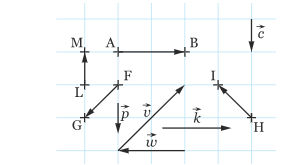
\includegraphics[width=0.95\linewidth]{ex27.png}
\end{center}
\begin{enumerate}
\item Repérer les vecteurs égaux, les vecteurs opposés et les vecteurs de même norme.
\item Quelle est l'image du point $F$ par la translation de vecteur $\Vj{LM}$~?
\item Par quelles translations le point $A$ est-il l'image du point $B$~?
\end{enumerate}
\end{Exo}

\begin{Exo}{Ex~28 p~185}{\starfull{diffgreen}\starempty\starempty}{Communiquer}
On considère la figure suivante composée de triangles équilatéraux. Recopier et compléter les phrases suivantes.
\begin{center}
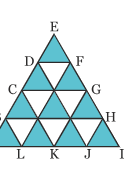
\includegraphics[width=0.75\linewidth]{ex28.png}
\end{center}
\begin{enumerate}
\item Le point $D$ a pour image le point \dots{} par la translation de vecteur $\Vj{G\dots}$.
\item $\dots=\dots$ signifie que \dots{} est l'image de \dots{} par la translation de vecteur \dots{}.
\end{enumerate}
\end{Exo}

\begin{Exo}{Ex~29 p~185}{\starempty\starfull{diffblue}\starempty}{Communiquer}
On considère un parallélogramme $ABCD$ de centre $O$ et le triangle équilatéral $BCE$. $G$, $H$ et $I$ sont les milieux respectifs de $[BE]$, de $[CE]$ et de $[BC]$.
\begin{enumerate}
\item Faire une figure à main levée.
\item Indiquer trois couples de vecteurs égaux deux à deux en justifiant à l'aide de propriétés vectorielles du cours.
\end{enumerate}
\end{Exo}

\begin{Exo}{Ex~30 p~185}{\starfull{diffgreen}\starempty\starempty}{Communiquer}
Voici les motifs d'un papier peint dont le pavage rappelle les \oe uvres de l'artiste Maurits Cornelis Escher (1898 -- 1972).
\begin{center}
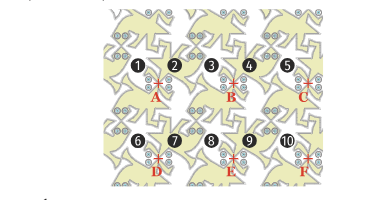
\includegraphics[width=0.85\linewidth]{ex30.png}
\end{center}
\begin{enumerate}
\item Écrire quatre phrases en utilisant l'expression \og est l'image de \fg. Par exemple~: \og La figure 8 est l'image de la figure 1 par la translation de vecteur $\Vj{AE}$. \fg
\item Écrire quatre phrases en utilisant l'expression \og a pour image \fg.
\end{enumerate}
\end{Exo}

\begin{Exo}{Ex~31 p~185}{\starempty\starfull{diffblue}\starempty}{Représenter}
On considère les vecteurs $\Vj{AB}$ et $\Vj{EF}$ et un point $C$.
\begin{center}
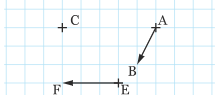
\includegraphics[width=0.7\linewidth]{ex31.png}
\end{center}
\begin{enumerate}
\item Reproduire la figure sur papier quadrillé.
\item Construire les points manquants.
\begin{enumerate}
\item[a.] $D$ tel que $\Vj{CD}=\Vj{AB}$
\item[b.] $G$ tel que $\Vj{CG}=\Vj{EF}$
\item[c.] $H$ tel que $\Vj{HC}=\Vj{AB}$
\item[d.] $I$ tel que $\Vj{IC}=\Vj{CG}$
\item[e.] $J$ tel que $\Vj{BJ}=\Vj{JC}$
\end{enumerate}
\end{enumerate}
\end{Exo}

\begin{Exo}{Ex~32 p~185}{\starfull{diffgreen}\starempty\starempty}{Représenter}
Reproduire la figure suivante sur papier pointé.
\begin{center}
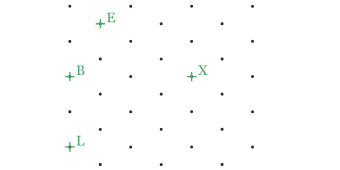
\includegraphics[width=0.55\linewidth]{ex32.png}
\end{center}
\begin{enumerate}
\item Construire les points $F$ et $A$, images de $E$ et $L$ par la translation de vecteur $\Vj{BX}$.
\item Construire les points $G$ et $H$, images de $E$ et $F$ par la translation de vecteur $\Vj{BL}$.
\item Tracer en traits pleins les segments $[BE]$, $[BX]$, $[BL]$, $[LA]$, $[XA]$, $[AH]$, $[FH]$, $[EF]$, $[XF]$ puis, en pointillés, les segments $[GE]$, $[GL]$ et $[GH]$.
\item Quel solide obtient-on~?
\end{enumerate}
\end{Exo}

\begin{Exo}{Ex~33 p~185}{\starempty\starfull{diffblue}\starempty}{Représenter}
On considère les points $A$, $B$, $C$, $I$ et $J$ suivants. Reproduire la figure et, en laissant les traits de construction, répondre aux questions suivantes.
\begin{center}
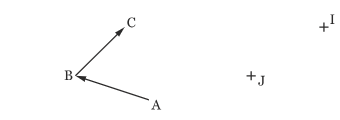
\includegraphics[width=0.7\linewidth]{ex33.png}
\end{center}
\begin{enumerate}
\item Construire les points $R$ et $S$, images de $I$ et $J$ par la translation de vecteur $\Vj{AB}$.
\item Construire les points $T$ et $U$, images de $R$ et $S$ par la translation de vecteur $\Vj{BC}$.
\item Par quelle translation le point $U$ est-il l'image du point $J$~?
\end{enumerate}
\end{Exo}

\begin{Exo}{Ex~35 p~185}{\starempty\starfull{diffblue}\starempty}{Raisonner}
On considère un parallélogramme $RSTU$ de centre $O$. On note $F$, l'image du point $S$ par la translation de vecteur $\Vj{UT}$ et $E$ l'image de $F$ par la translation de vecteur $\Vj{RU}$.
\begin{enumerate}
\item Faire une figure.
\item À l'aide des propriétés vectorielles, démontrer que $RSET$ est un parallélogramme.
\end{enumerate}
\end{Exo}

\begin{Exo}{Ex~38 p~186}{\starfull{diffgreen}\starempty\starempty}{Raisonner}
Soit $ABC$ un triangle quelconque. On note $I$ le milieu de $[AB]$.
\begin{center}
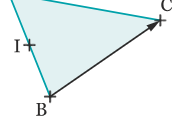
\includegraphics[width=0.65\linewidth]{ex38.png}
\end{center}
\begin{enumerate}
\item Reproduire la figure et construire le point $I'$, image de $I$ par la translation de vecteur $\Vj{BC}$.
\item Construire le point $A'$, image de $A$ par la translation de vecteur $\Vj{I'I}$.
\item Démontrer que $A'BCA$ est un parallélogramme.
\item En déduire que $\Vj{A'I}=\Vj{IC}$.
\end{enumerate}
\end{Exo}

\begin{Exo}{Ex~39 p~186}{\starfull{diffgreen}\starempty\starempty}{Représenter}
On considère les vecteurs suivants représentés sur du papier quadrillé.
\begin{center}
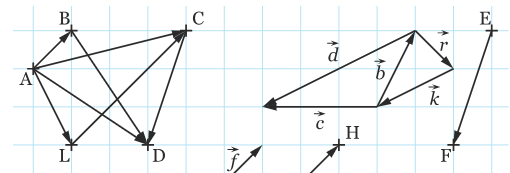
\includegraphics[width=0.95\linewidth]{ex39.png}
\end{center}
\begin{enumerate}
\item Écrire cinq sommes de vecteurs traduisant la relation de Chasles.
\item Transformer les expressions suivantes de façon à faire apparaître la relation de Chasles et à déterminer le vecteur somme.
\begin{multicols}{2}
\begin{enumerate}
\item[a.] $\Vj{BC}+\Vj{EF}$
\item[b.] $\Vj{EF}+\Vj{LC}$
\item[c.] $\Vj{GH}+\Vj{BC}$
\item[d.] $\Vj{BC}+\vec b$
\end{enumerate}
\end{multicols}
\end{enumerate}
\end{Exo}

\begin{Exo}{Ex~42 p~187}{\starfull{diffgreen}\starempty\starempty}{Représenter}
On considère les figures suivantes.
\begin{center}
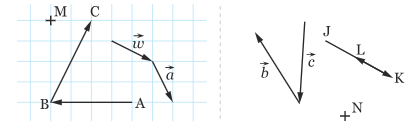
\includegraphics[width=0.95\linewidth]{ex42-p187.png}
\end{center}
\begin{enumerate}
\item Reproduire les figures.
\item Tracer les vecteurs~: $\Vj{AB}+\Vj{BC}$, $\vec w+\vec a$, $\vec b+\vec c$, $\Vj{JK}+\Vj{KL}$.
\item Placer les points $P$, $R$, $S$ et $T$ tels que~:
\begin{enumerate}
\item[a.] $\Vj{MR}$ soit égal au vecteur $\vec w+\vec a$.
\item[b.] $\Vj{NS}$ soit égal au vecteur somme $\vec b+\vec c$.
\item[c.] $\Vj{NT}$ soit égal au vecteur somme $\Vj{JK}+\Vj{KL}$.
\end{enumerate}
\end{enumerate}
\end{Exo}

\begin{Exo}{Ex~43 p~187}{\starempty\starfull{diffblue}\starempty}{Représenter}
On considère les vecteurs suivants.
\begin{center}
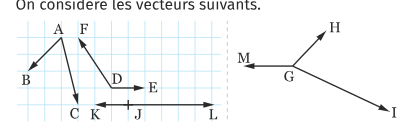
\includegraphics[width=0.95\linewidth]{ex43.png}
\end{center}
Tracer les sommes des vecteurs définies par~:
\begin{multicols}{2}
\begin{enumerate}
\item[a.] $\Vj{AP}=\Vj{AB}+\Vj{AC}$
\item[b.] $\Vj{DR}=\Vj{DE}+\Vj{DF}$
\item[c.] $\Vj{JT}=\Vj{JK}+\Vj{JL}$
\item[d.] $\Vj{GW}=\Vj{GH}+\Vj{GM}$
\item[e.] $\Vj{GX}=\Vj{GM}+\Vj{GI}$
\item[f.] $\Vj{GZ}=\Vj{GI}+\Vj{GH}$
\end{enumerate}
\end{multicols}
\end{Exo}

\begin{Exo}{Ex~45 p~187}{\starempty\starfull{diffblue}\starempty}{Représenter}
On considère les vecteurs suivants.
\begin{center}
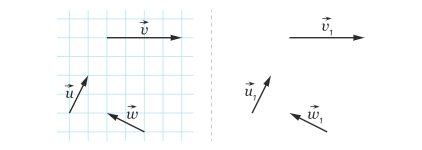
\includegraphics[width=0.95\linewidth]{ex45-p187.png}
\end{center}
\begin{enumerate}
\item Reproduire le quadrillage (figure de gauche) et tracer les sommes des vecteurs définies par~:
\begin{enumerate}
\item[a.] $\vec a=\vec u+\vec v$
\item[b.] $\vec b=\vec u+\vec w$
\item[c.] $\vec c=\vec v+\vec w$
\end{enumerate}
\item Reproduire la figure de droite et, à l'aide des instruments usuels, tracer les sommes des vecteurs définies par~:
\begin{enumerate}
\item[a.] $\vec{a_1}=\vec{u_1}+\vec{v_1}$
\item[b.] $\vec{b_1}=\vec{u_1}+\vec{w_1}$
\item[c.] $\vec{c_1}=\vec{v_1}+\vec{w_1}$
\end{enumerate}
\end{enumerate}
\end{Exo}

\begin{Exo}{Ex~68 p~191}{\starfull{diffgreen}\starempty\starempty}{Représenter}
On considère l'hélicoptère ci-dessous sur lequel sont exercées deux forces.
\begin{center}
\begin{tikzpicture}[scale=0.9]
\draw[thick] (-1.5,0) .. controls (-1.5,0.55) and (-0.8,0.75) .. (0.3,0.7)
 .. controls (0.9,0.68) and (1.1,0.45) .. (1.0,0.15)
 .. controls (0.9,-0.15) and (0.2,-0.3) .. (-0.7,-0.25)
 .. controls (-1.2,-0.22) and (-1.5,-0.1) .. (-1.5,0) -- cycle;
\draw[thick] (1.0,0.15) -- (2.6,0.55);
\draw[thick] (2.5,0.5) -- (2.75,0.75); \draw[thick] (2.5,0.5) -- (2.7,0.3);
\draw[thick] (-1.9,0.95) -- (1.9,0.95);
\draw[thick] (0,0.7) -- (0,0.95);
\draw[thick] (-1.1,-0.55) -- (0.7,-0.55);
\draw[thick] (-1.0,-0.25) -- (-1.0,-0.55); \draw[thick] (0.5,-0.15) -- (0.5,-0.55);
\coordinate (G) at (-0.2,0.35);
\draw[thick] ($(G)+(-0.12,0)$) -- ($(G)+(0.12,0)$);
\draw[thick] ($(G)+(0,-0.12)$) -- ($(G)+(0,0.12)$);
\draw[-{Stealth},thick,orange] (G) -- ++(0.5,1.3);
\end{tikzpicture}
\end{center}
La rotation des pales qui permet à l'hélicoptère de voler est représentée par un vecteur dont la norme est 2U (2 unités). La force de gravitation qui attire l'hélicoptère vers le bas est représentée par un vecteur vertical orienté vers le bas et dont la norme est 1U (1 unité). L'angle formé par les deux vecteurs est de 150\textdegree.
\begin{enumerate}
\item Faire une figure en prenant 5~cm pour unité.
\item Le déplacement de l'hélicoptère est décrit par la somme des deux forces exercées.
\begin{enumerate}
\item[a.] Construire le vecteur représentant le déplacement.
\item[b.] Mesurer sa norme à la règle pour avoir sa valeur en cm et en déduire sa valeur en U.
\end{enumerate}
\item La pilote de l'hélicoptère souhaite faire du sur-place. Pour cela, on peut exercer une troisième force ayant la même origine que les deux autres.
\begin{enumerate}
\item[a.] Quelle est la somme des trois forces exercées sur l'hélicoptère lorsqu'il fait du sur-place~?
\item[b.] Représenter cette force.
\end{enumerate}
\end{enumerate}
\end{Exo}

\begin{Exo}{Ex~69 p~191}{\starfull{diffgreen}\starempty\starempty}{Représenter}
Une péniche est tirée par deux personnes à l'aide de cordes sur le chemin de halage qui longe le canal. Les vecteurs décrivent les deux forces en termes de sens, de direction et d'intensité.
\begin{center}
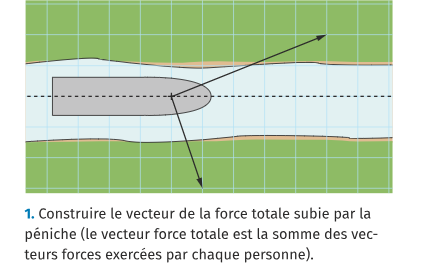
\includegraphics[width=0.95\linewidth]{ex69.png}
\end{center}
\begin{enumerate}
\item Construire le vecteur de la force totale subie par la péniche (le vecteur force totale est la somme des vecteurs forces exercées par chaque personne). Y a-t-il un problème à terme~?
\item Modifier une des deux forces pour que la péniche poursuive sa course dans la même direction sans heurter la berge.
\end{enumerate}
\end{Exo}

\begin{Exo}{Ex~71 p~192}{\starempty\starfull{diffblue}\starempty}{Chercher}
Pour tester un nouveau prototype de bateau à moteur, les ingénieurs réalisent des tests sur maquette en piscine. En présence d'un courant latéral simulé par des buses, ils souhaitent étudier le cap à donner au bateau pour qu'il atteigne le port, noté $P$, en ligne droite. On note $\vec{V_m}$ le vecteur vitesse de la maquette sur l'eau, $\vec{V_c}$ celle du courant simulé en piscine et $\vec{V_b}$ celle de la maquette par rapport au bord.
\begin{center}
\begin{tikzpicture}[scale=0.5]
\draw[thin,cyan!25] (0,0) grid (9,7);
\fill[cyan!10] (0,0) -- (0,6) -- (6,6) arc[start angle=90,end angle=0,radius=3] -- (9,0) -- cycle;
\draw[thick] (0,0) -- (0,6) -- (6,6) arc[start angle=90,end angle=0,radius=3] -- (9,0) -- cycle;
\draw[thick] (0,3.6) -- (-0.7,3.6) -- (-0.7,2.6) -- (0,2.6);
\node[left] at (-0.7,3.1) {$P$};
\node[right,font=\scriptsize] at (0.2,6.4) {Piscine d'essai};
\fill[red] (2.6,2.6) circle (2.2pt);
\node[below,font=\scriptsize] at (2.9,2.2) {Maquette de test};
\draw[-{Stealth},thick,orange] (2.6,2.6) -- ++(-1,1.3) node[midway,left,font=\scriptsize]{$\vec{V_m}$};
\draw[-{Stealth},thick,blue] (6.5,5) -- ++(-1.3,-0.9);
\draw[-{Stealth},thick,blue] (7.3,4) -- ++(-1.3,-0.9);
\draw[-{Stealth},thick,blue] (8,3) -- ++(-1.3,-0.9) node[midway,below,font=\scriptsize]{$\vec{V_c}$};
\draw[-{Stealth},thick,dashed] (2.6,2.6) -- (0,3.1) node[midway,above,font=\scriptsize]{?};
\end{tikzpicture}
\end{center}
\begin{enumerate}
\item On admet que $\vec{V_b}=\vec{V_m}+\vec{V_c}$. Quelle direction sur l'eau doit prendre le bateau pour atteindre le point $P$~?
\item Dans le cas où le bateau se positionne face au courant, à quelle condition sera-t-il capable de le remonter~?
\end{enumerate}
\end{Exo}

\begin{Exo}{Ex~72 p~192}{\starempty\starfull{diffblue}\starempty}{Chercher}
Dans un triangle, on appelle \textbf{médiane} issue d'un sommet la droite qui passe par ce sommet et par le milieu du côté opposé. On admet que les trois médianes d'un triangle sont concourantes en un point appelé \textbf{centre de gravité}. On souhaite établir une relation vectorielle caractéristique de ce point particulier.
\begin{center}
\begin{tikzpicture}[scale=1.1]
\coordinate (A) at (0,2.2); \coordinate (B) at (-1.6,-1.2); \coordinate (C) at (2.4,0.4);
\coordinate (D) at ($(A)!0.5!(B)$); \coordinate (E) at ($(A)!0.5!(C)$); \coordinate (F) at ($(B)!0.5!(C)$);
\coordinate (G) at ($(A)!0.6667!(F)$);
\draw[thick,teal!40,fill=teal!12] (A) -- (B) -- (C) -- cycle;
\draw[dashed] (A) -- (F); \draw[dashed] (B) -- (E); \draw[dashed] (C) -- (D);
\fill (A) circle(1.3pt) (B) circle(1.3pt) (C) circle(1.3pt) (D) circle(1.3pt) (E) circle(1.3pt) (F) circle(1.3pt) (G) circle(1.3pt);
\node[above] at (A) {$A$}; \node[below left] at (B) {$B$}; \node[right] at (C) {$C$};
\node[left] at (D) {$D$}; \node[above right] at (E) {$E$}; \node[below] at (F) {$F$};
\node[above right] at (G) {$G$};
\end{tikzpicture}
\end{center}
\begin{enumerate}
\item Découper dans du carton un triangle $ABC$ de dimension quelconque puis chercher par tâtonnement le point d'équilibre de ce triangle en utilisant la pointe d'un compas comme support.
\item Tracer les trois médianes du triangle construit et vérifier que le point d'équilibre trouvé au compas est le centre de gravité.
\item Dans GeoGebra, reproduire la figure ci-dessus où $D$, $E$ et $F$ sont les milieux respectifs de $[AB]$, $[AC]$ et $[BC]$. Représenter les vecteurs $\Vj{GA}$, $\Vj{GB}$ et $\Vj{GC}$.
\item Construire le vecteur somme $\Vj{GA}+\Vj{GB}+\Vj{GC}$. Que constate-t-on~?
\item Rédiger la propriété observée.
\end{enumerate}
\end{Exo}

\begin{Exo}{Ex~19 p~207}{\starfull{diffgreen}\starempty\starempty}{Chercher}
Parmi les vecteurs du repère, lesquels sont colinéaires~?
\begin{center}
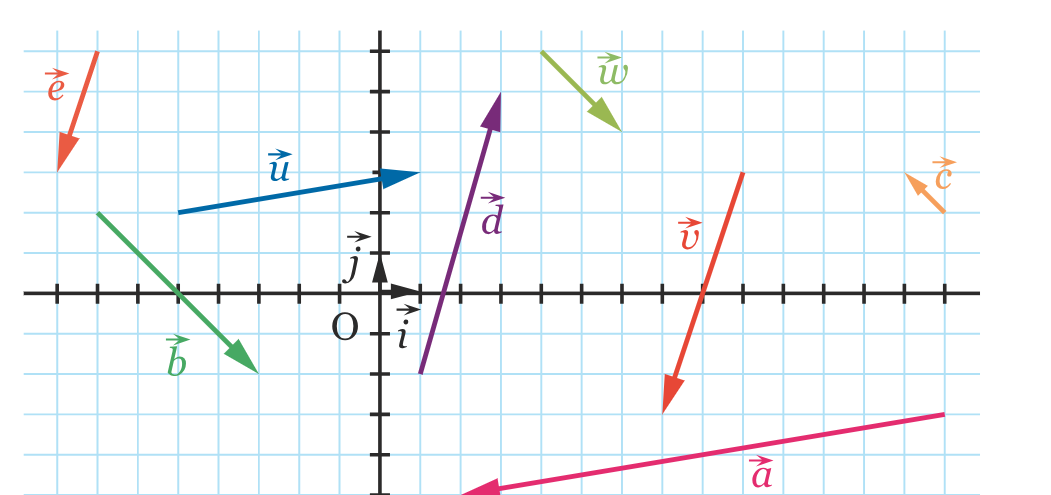
\includegraphics[width=0.95\linewidth]{ex19.png}
\end{center}
\end{Exo}

\begin{Exo}{Ex~41 p~208 à 210}{\starempty\starfull{diffblue}\starempty}{Chercher}
Quelques points ont été placés sur l'axe ci-dessous.
\begin{center}
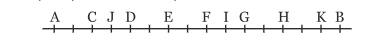
\includegraphics[width=0.95\linewidth]{ex41.png}
\end{center}
\begin{enumerate}
\item Recopier et compléter les égalités suivantes avec des nombres réels.
\begin{multicols}{2}
\begin{enumerate}
\item[a.] $\Vj{ED}=\dots\Vj{CJ}$
\item[b.] $\Vj{FH}=\dots\Vj{KB}$
\item[c.] $\Vj{CD}=\dots\Vj{AK}$
\item[d.] $\Vj{DE}=\dots\Vj{FC}$
\end{enumerate}
\end{multicols}
\item Recopier et compléter l'égalité $\Vj{GF}=\dots\Vj{AJ}$ et en déduire le coefficient $k$ tel que $\Vj{AJ}=k\Vj{GF}$.
\item Quelle est l'image du point $E$ par la translation de vecteur $2\Vj{AD}$~?
\item Quelle est l'image du point $F$ par la translation de vecteur $-\dfrac12\Vj{EC}$~?
\end{enumerate}
\end{Exo}

\begin{Exo}{Ex~42 p~208 à 210}{\starfull{diffgreen}\starempty\starempty}{Représenter}
Reproduire la figure suivante et construire les points $C$ et $D$ tels que $\Vj{RC}=\dfrac14\vec u$ et $\Vj{DR}=-\dfrac32\vec u$.
\begin{center}
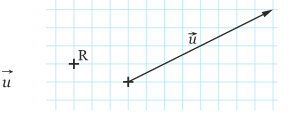
\includegraphics[width=0.6\linewidth]{ex42-p208.png}
\end{center}
\end{Exo}

\begin{Exo}{Ex~44 p~208 à 210}{\starfull{diffgreen}\starempty\starempty}{Représenter}
\begin{enumerate}
\item Soient $A$, $O$ et $N$ trois points du plan alignés comme sur la figure ci-contre. Écrire une phrase incluant ces trois points et le mot \og homothétie \fg.
\item Reproduire la figure et construire le point $B$ tel que $\Vj{AB}=-2\Vj{ON}$ et le point $C$ tel que $\Vj{BC}=3\Vj{ON}$.
\end{enumerate}
\begin{center}
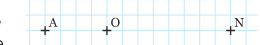
\includegraphics[width=0.6\linewidth]{ex44-p208a.png}\\[6pt]
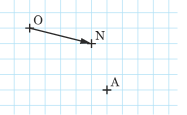
\includegraphics[width=0.4\linewidth]{ex44-p208b.png}
\end{center}
\end{Exo}

\begin{Exo}{Ex~45 p~208 à 210}{\starempty\starempty\starfull{diffred}}{Représenter}
Reproduire la figure ci-dessous.
\begin{center}
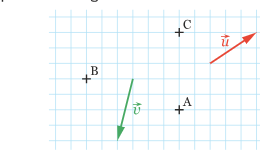
\includegraphics[width=0.55\linewidth]{ex45-p208.png}
\end{center}
\begin{enumerate}
\item Construire le point $D$ tel que $\Vj{AD}=2\vec u-\vec v$.
\item Construire le point $F$ tel que $\Vj{BF}=-2\vec v-3\Vj{AB}$.
\item Construire le point $E$ tel que $\Vj{CE}=\Vj{AB}-\Vj{FB}+\vec v-\dfrac13\vec u$.
\end{enumerate}
\end{Exo}

\begin{Exo}{Ex~61 p~210}{\starfull{diffgreen}\starempty\starempty}{Chercher}
Les vecteurs $\vec u$, $\vec v$, $\vec w$, $\vec k$, $\vec r$ et $\vec s$ sont représentés dans le repère ci-dessous.
\begin{center}
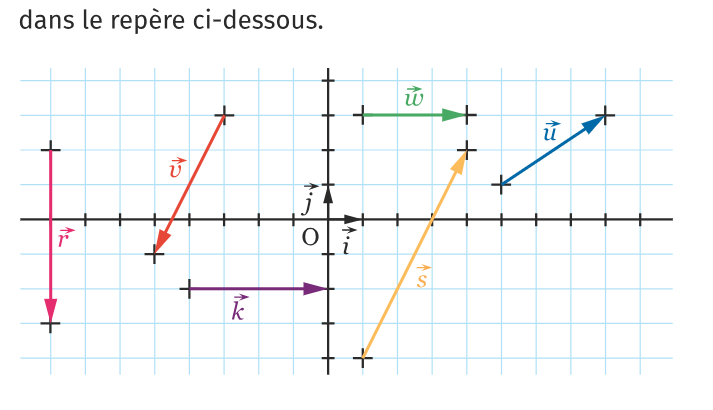
\includegraphics[width=0.95\linewidth]{ex61.png}
\end{center}
Quels vecteurs sont colinéaires~? Déterminer la relation liant ces vecteurs.
\end{Exo}

\begin{Exo}{Ex~74 p~212}{\starempty\starfull{diffblue}\starempty}{Chercher}
Reproduire la figure ci-dessous.
\begin{center}
\begin{tikzpicture}[scale=0.55]
\draw[thin,cyan!30] (0,0) grid (6,4.5);
\coordinate (C) at (2.5,3.7); \coordinate (A) at (1.5,2.2); \coordinate (B) at (3,1.7);
\node[above] at (C) {$+\,C$}; \node[left] at (A) {$+\,A$}; \node[below right] at (B) {$+\,B$};
\fill (C) circle(1.3pt) (A) circle(1.3pt) (B) circle(1.3pt);
\end{tikzpicture}
\end{center}
\begin{enumerate}
\item Construire les points $E$ et $F$ tels que~: $\Vj{AE}=2\Vj{AB}+\dfrac12\Vj{BC}$ et $\Vj{AF}=2\Vj{AC}-2\Vj{BC}$.
\item Démontrer que $\Vj{EF}=-\dfrac12\Vj{BC}$.
\item Que peut-on en déduire à propos des droites $(EF)$ et $(BC)$~?
\end{enumerate}
\end{Exo}

\begin{Exo}{Ex~75 p~212}{\starempty\starempty\starfull{diffred}}{Chercher}
Reproduire la figure ci-dessous.
\begin{center}
\begin{tikzpicture}[scale=0.55]
\draw[thin,cyan!30] (0,0) grid (6,4.5);
\coordinate (B) at (1.5,3.7); \coordinate (A) at (3.3,1.9); \coordinate (C) at (1.8,0.9);
\node[above] at (B) {$+\,B$}; \node[right] at (A) {$+\,A$}; \node[below] at (C) {$+\,C$};
\fill (B) circle(1.3pt) (A) circle(1.3pt) (C) circle(1.3pt);
\end{tikzpicture}
\end{center}
\begin{enumerate}
\item Construire le point $F$ tel que $\Vj{AF}=2\Vj{AC}-2\Vj{BC}$.
\item Quelle relation existe-t-il entre les points $B$, $A$ et $F$~? Justifier.
\end{enumerate}
\end{Exo}

\end{multicols}

\end{document}
